
\chapter{APT, Logging and Forensic}
\newpage

\section{lecture}

\subsection{Advanced Persistent Threat (APT)}
APT levels are typically categorized into 3 tiers:

\begin{itemize}
  \item APT Level 1:
  \begin{itemize}
    \tightlist
		\item Nation-state actors
		\item Highly sophisticated
		\item Custom malware/tools
		\item Multiple zero-days
		\item Examples: Cozy Bear, Fancy Bear
  \end{itemize}

  \item APT Level 2:
  \begin{itemize}
    \tightlist
		\item Nation-states/Large criminal groups
		\item Known exploits/tools
		\item Some custom capabilities
		\item Examples: FIN7, Carbanak
  \end{itemize}

  \item APT Level 3:
  \begin{itemize}
    \tightlist
		\item Criminal organizations
		\item Commercial tools
		\item Known TTPs
		\item Limited resources
		\item Examples: Various cybercrime groups
  \end{itemize}

  \item Key differences between levels:
  \begin{itemize}
    \tightlist
		\item Resource availability
		\item Technical sophistication
		\item Persistence capability
		\item Infrastructure complexity
		\item Target selection
  \end{itemize}
\end{itemize}

\subsection{Logging}

\textbf{Logging Services}
Common logging services:

\begin{itemize}
  \item Enterprise SIEM:
  \begin{itemize}
    \tightlist
		\item Splunk
		\item ELK Stack
		\item QRadar
		\item LogRhythm
		\item ArcSight
  \end{itemize}

  \item Cloud-native:
  \begin{itemize}
    \tightlist
		\item AWS CloudWatch
		\item Azure Monitor
		\item Google Cloud Logging
		\item Datadog
		\item New Relic
  \end{itemize}

  \item Open Source:
  \begin{itemize}
    \tightlist
		\item Graylog
		\item Loki
		\item Fluentd
		\item Logstash
		\item rsyslog
  \end{itemize}

  \item Features to consider:
  \begin{itemize}
    \tightlist
		\item Real-time monitoring
		\item Search capabilities
		\item Alert mechanisms 
		\item Retention periods
		\item Compliance support
		\item Integration options
  \end{itemize}
\end{itemize}


\textbf{Key logging categories for security analysis:}
\begin{itemize}
  \item Network:
  \begin{itemize}
    \tightlist
		\item NetFlow/traffic data
		\item DNS queries/responses
		\item HTTP/HTTPS requests
		\item IDS/IPS alerts
		\item Firewall logs
  \end{itemize}

  \item System:
  \begin{itemize}
    \tightlist
		\item Authentication attempts
		\item Process creation
		\item File access/changes
		\item Registry modifications
		\item Service starts/stops
  \end{itemize}

  \item Application:
  \begin{itemize}
    \tightlist
		\item API calls
		\item Database queries
		\item User actions
		\item Error messages
		\item Configuration changes
  \end{itemize}

  \item Forensic Uses:
  \begin{itemize}
    \tightlist
		\item Establish attack timeline
		\item Identify initial access
		\item Track lateral movement
		\item Document data exfiltration
		\item Determine persistence mechanisms
		\item Map attacker infrastructure
		\item Identify compromised accounts
  \end{itemize}

  \item Critical Fields:
  \begin{itemize}
    \tightlist
		\item Timestamps
		\item Source/destination IPs
		\item User accounts
		\item Process IDs
		\item File hashes
		\item Command lines
		\item Network ports
  \end{itemize}
\end{itemize}

\textbf{Lookup Services}
\begin{itemize}
  \item \textbf{Block\&Black}: Threat intelligence sharing platform. Tracks malicious IPs, domains, malware signatures.
  \item \textbf{Mandiant}: Advanced threat research and incident response services. Provides detailed threat actor profiles and IoC tracking
  \item \textbf{ZEUS TRACKER}: Monitors Zeus botnet activity. Tracks C2 servers, infected IPs, malware variants.
  \item \textbf{Maleware Hash}: Database services for identifying malware through cryptographic hashes. Helps verify file authenticity/maliciousness.
  \item \textbf{OpenIOC}: Framework for sharing threat intelligence and indicators of compromise. Used for describing attack patterns.
  \item \textbf{IP Reputation}: Services tracking IP addresses associated with malicious activity. Examples: AbuseIPDB, IBM X-Force, VirusTotal IP lookups.
\end{itemize}

\subsection{Cyber Security tools and frameworks for logging and forensic}
\textbf{SIEM}
Security Information and Event Management solutions are responsible for collecting log and event data from various sources such as network, servers and applications and aggregating, identifying, categorizing and analyzing it in real time. With a SIEM solution, security problems should be detected automatically as well as the ability to send an alert
\begin{itemize}
  \item Enables pattern search in log data for indicators of a cyberattack (IOC)
  \item Enables correlation of event information and identifies abnormal activity
  \item Alerts according to defined alert rules
\end{itemize}

\textbf{SOAR}
SOAR also collects data from various sources similar to a SIEM, but SOAR supports the incident responder in managing the crisis. SOAR enables automated intervention when a security incident occurs. A SOAR system also supports the incident responder in rolling out security countermeasures (Active Directory).

\begin{itemize}
  \item SOAR (Security Orchestration, Automation and Response):
  \item Alert Investigation
  \item Orchestration
  \item Automation workflow
	\item Automates security operations workflows and incident response
	\item Integrates with other security tools for coordinated actions
	\item Reduces manual intervention in repetitive security tasks
\end{itemize}

\textbf{EDR}
Endpoint detection and response (EDR), also known as endpoint threat detection and response (ETDR), is an integrated endpoint security solution that combines real-time continuous monitoring and collection of endpoint data with rules-based automated response and analysis capabilities
\begin{itemize}
	\item Monitors endpoints (computers, servers, mobile devices) for suspicious activity
	\item Provides advanced threat detection and incident investigation capabilities
	\item Can automatically respond to detected threats
\end{itemize}

\begin{itemize}
  \item CIRT (Computer Incident Response Team):
  \begin{itemize}
    \tightlist
		\item Group responsible for handling cybersecurity incidents
		\item Coordinates response efforts across organization
		\item Investigates breaches and implements recovery procedures
  \end{itemize}

  \item YARA:
  \begin{itemize}
    \tightlist
		\item Pattern matching tool for malware identification
		\item Uses rules to identify and classify malware samples
		\item Widely used in threat hunting and malware analysis
  \end{itemize}
\end{itemize}

\textbf{Wazuh}
Wazuh is an open source security platform that focuses on infrastructure monitoring, security risk detection and incident response in the sense of a SIEM and EDR (Endpoint Detection \& Response).

The so-called Wazuh agent is installed on the machines to be monitored and communicates with the Wazuh manager, which is installed on a server. To ensure that the data is clearly represented, it is further sent to components of Elastic Stack and displayed in a dashboard using Kibana. Translated with www.DeepL.com/Translator (free version)

\textbf{Evolution}
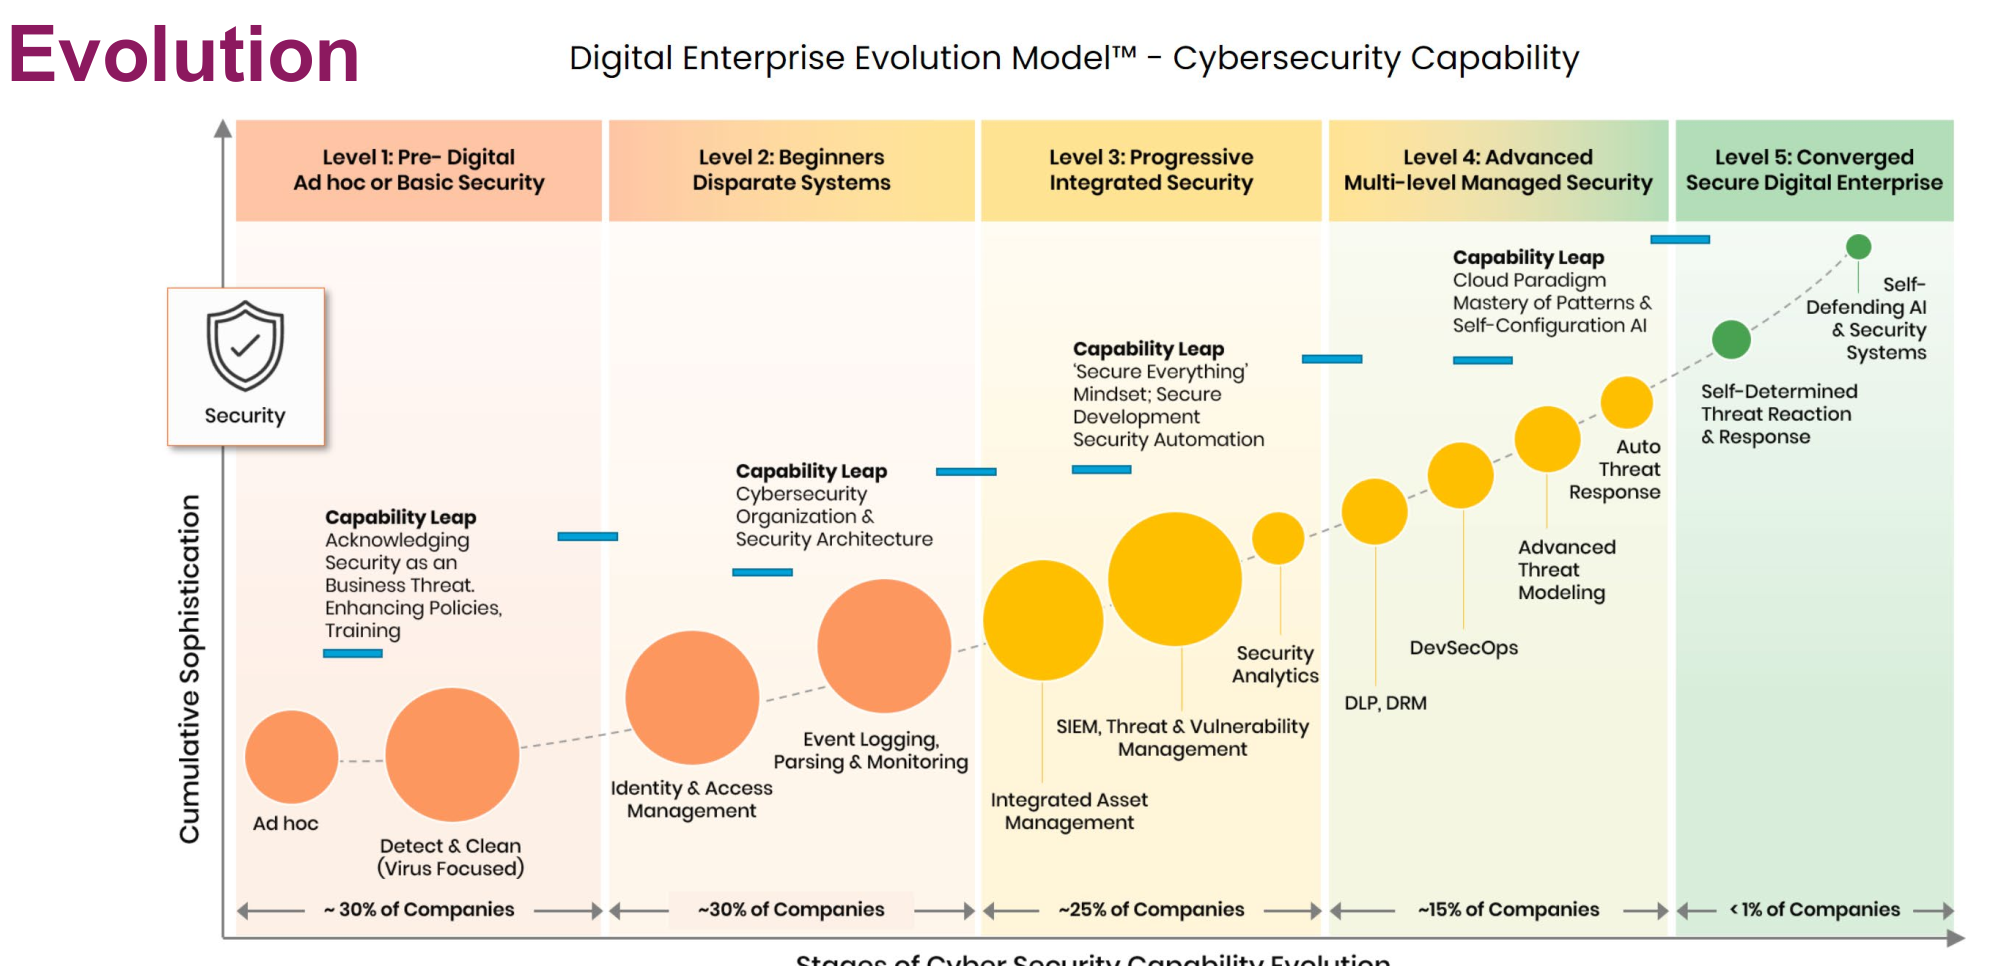
\includegraphics[width=\textwidth]{resources/04-evolution-cybersecurity-capabilities.png}

These tools often work together in an organization's security infrastructure, with SIEM collecting data, SOAR automating responses, EDR protecting endpoints, CIRT managing incidents, and YARA helping identify threats.

\subsubsection{Interaction SIEM, EDR, SOAR}
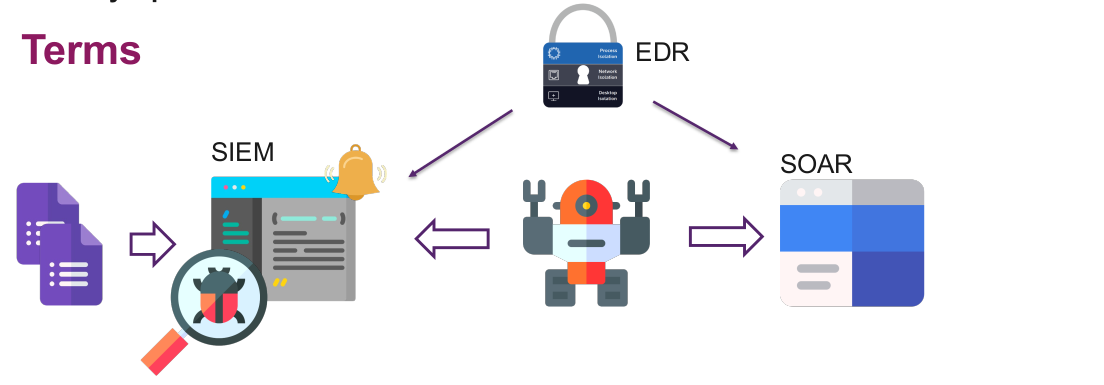
\includegraphics[width=\textwidth]{resources/04-interaction-security-operation-center.png}
The three components (SIEM, EDR, and SOAR) interact in a cybersecurity workflow:
\begin{enumerate}
	\item SIEM collects security logs and alerts from across the network and acts as the central monitoring system.
	\item EDR monitors endpoints and sends detailed threat data to SIEM about detected malicious activities or anomalies.
	\item SOAR receives alerts from SIEM, then:
  \begin{itemize}
    \tightlist
		\item Automatically investigates threats
		\item Orchestrates response actions
		\item Initiates predetermined playbooks
		\item Can instruct EDR to take actions like isolating infected endpoints
  \end{itemize}
  \subsubsection*{This creates a cycle where:}
  \begin{itemize}
    \tightlist
		\item EDR detects threats
		\item SIEM aggregates and analyzes the data
		\item SOAR automates the response
		\item SOAR can trigger EDR actions to contain threats
  \end{itemize}
\end{enumerate}
This integration enables faster threat detection and automated incident response across the security infrastructure.

\subsection{Velociraptor}

A powerful DFIR technique is searching bulk data for patterns
\begin{itemize}
  \item Searching for CC data in process memory
  \item Searching for URLs in process memory
  \item Searching binaries for malware signatures
  \item Searching registry for patterns
\end{itemize}
Bulk searching helps to identify evidence without needing to parse file formats

\begin{itemize}
  \item Live forensic analysis across enterprise networks
  \item Collection of system artifacts and telemetry
  \item Advanced threat hunting using VQL (Velociraptor Query Language)
  \item Scalable deployment for large-scale investigations
  \item Custom artifact creation for specific investigation needs
  \subsubsection*{Key features:}
  \item Agentless or agent-based deployment options
  \item Cross-platform support (Windows, Linux, macOS)
  \item Efficient resource usage even at scale
  \item Integration with other security tools like SIEM
  \item Built-in artifact exchange for community sharing
\end{itemize}

\subsection{YARA}
YARA is a pattern matching tool used to identify and classify malware. It uses rule-based pattern matching to detect malicious content in files.
\begin{itemize}
  \item YARA is a powerful keyword scanner
  \item Uses rules designed to identify binary patterns in bulk data
  \item YARA is optimized to scan for many rules simultaneously.
  \item Velociraptor supports YARA scanning of bulk data (via accessors) and memory.
\end{itemize}

\begin{itemize}
  \subsubsection*{Key capabilities:}
	\item Creates rules to identify malware variants
	\item Matches binary patterns and strings
	\item Supports complex conditions and regular expressions
	\item Integrates with other security tools
	\item Used for malware hunting and classification

  \subsubsection*{Example YARA rule structure:}
  \item \begin{lstlisting}
    rule MalwareExample {
      strings:
          $suspicious_string = "malicious_pattern"
          $hex_pattern = { 4D 5A 90 00 }
      condition:
          $suspicious_string and $hex_pattern
    }
    \end{lstlisting}

  \subsubsection*{Common uses:}
	\item Malware classification
	\item Threat hunting
	\item Incident response
	\item Malware family identification
	\item Automated malware analysis
\end{itemize}

\subsection{CIRT/CSIRT}

\subsubsection*{CERT}
\begin{itemize}
  \item Computer Emergency Response Team
  \item Trademark
  \item Imprecise
\end{itemize}

\subsubsection*{CSIRT}
A CSIRT is a team of IT security experts whose main business is to respond to computer security incidents. It provides the necessary services to handle them and support their constituents to recover from breaches.

\subsection{Incident Response}
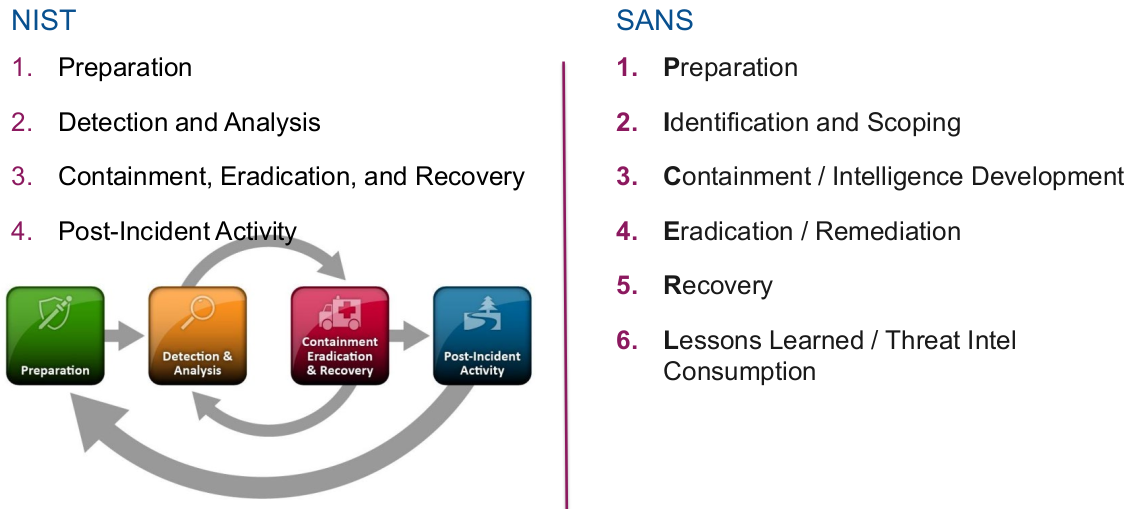
\includegraphics[width=\textwidth]{resources/04-incident-reponse.png}
Both NIST and SANS provide frameworks for incident response, with some key differences:
\begin{itemize}
  \subsubsection*{NIST Framework (4 phases):}
  \item Preparation: Establish policies, procedures, team structure
  \item Detection/Analysis: Identify and investigate incidents
  \item Containment/Eradication/Recovery: Stop incident spread, remove threats, restore systems
  \item Post-Incident Activity: Document lessons, improve processes
  \subsubsection*{SANS Framework (6 phases):}
  \item Preparation: Similar to NIST
  \item Identification/Scoping: Determine incident scope and impact
  \item Containment/Intelligence: Isolate affected systems, gather threat data
  \item Eradication/Remediation: Remove threat, fix vulnerabilities
  \item Recovery: Restore systems to normal operation
  \item Lessons Learned: Document findings, update procedures
\end{itemize}
Key Difference: SANS separates containment, eradication, and recovery into distinct phases and adds threat intelligence gathering, while NIST combines them into one phase.

\subsubsection*{Indicator of Compromise (IOC)}
Indicators of Compromise (IOCs) define characteristics of an incident in a structured manner. They have the goal to describe, communicate and find artifacts related to incidents.

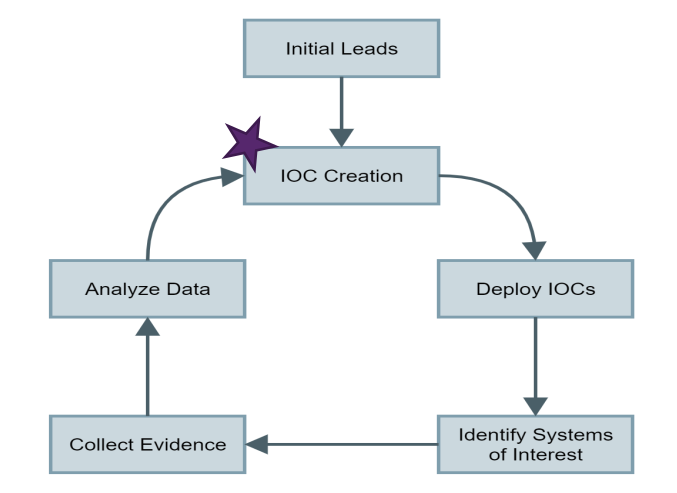
\includegraphics[width=\textwidth]{resources/04-ioc.png}
\begin{enumerate}
  \item Initial Leads $\rightarrow$ IOC Creation: Starting point for threat investigation
  \item IOC Creation $\rightarrow$ Deploy IOCs: Convert threat data into usable detection rules
  \item Deploy IOCs $\rightarrow$ Identify Systems: Find potentially compromised systems
  \item Identify Systems $\rightarrow$ Collect Evidence: Gather data from identified systems
  \item Collect Evidence $\rightarrow$ Analyze Data: Examine collected evidence
  \item Analyze Data $\rightarrow$ IOC Creation: Refine IOCs based on findings
\end{enumerate}
This creates a continuous cycle where threat detection improves through iteration and evidence analysis.
The purple star at IOC Creation indicates it's a critical phase where accuracy is essential. \\

\begin{itemize}
  \subsubsection*{Host-based IOC formats}
  \item YARA: Pattern matching for malware detection
  \item STIX/TAXII: Structured threat intel exchange (replaced Mitre's CybOX)
  \item Mandiant's OpenIOC: XML-based IOC format
  \subsubsection*{Network-based IOC formats}
  \item Snort rules: Network-based threat detection signatures
  \subsubsection*{These formats are designed for different use cases:}
  \item YARA for file analysis
  \item STIX/TAXII for threat intel sharing
  \item OpenIOC for endpoint threats
  \item Snort for network traffic analysis
\end{itemize}

\section{exercise}
